\pdfoutput=1
\documentclass[a4paper,pdflatex,ja=standard]{bxjsarticle}

% ---Setting about the geometry of the document----
% \usepackage{a4wide}
% \pagestyle{empty}

% ---Physics and Math Packages---
\usepackage{amssymb,amsfonts,amsthm,mathtools}
\usepackage{physics,braket,bm}

% ---underline---
\usepackage{ulem}

% --- sorround the texts or equations
% \usepackage{fancybox,ascmac}

% ---settings of theorem environment---
% \usepackage{amsthm}
% \theoremstyle{definition}

% ---settings of proof environment---
% \renewcommand{\proofname}{\textbf{証明}}
% \renewcommand{\qedsymbol}{$\blacksquare$}

% ---Ignore the Warnings---
\usepackage{silence}
\WarningFilter{latexfont}{Some font shapes,Font shape}

% ---Insert the figure (If insert the `draft' at the option, the process becomes faster)---
\usepackage{graphicx}
% \usepackage{subcaption}

% ----Add a link to a text---
\usepackage{url}
\usepackage{xcolor,hyperref}
\hypersetup{colorlinks=true,citecolor=orange,linkcolor=blue,urlcolor=magenta}
\usepackage{bxcjkjatype}

% ---Tikz---
\usepackage{tikz,pgf,pgfplots,circuitikz}
\pgfplotsset{compat=1.15}
\usetikzlibrary{intersections,arrows.meta,angles,calc,3d,decorations.pathmorphing}

% ---Add the section number to the equation, figure, and table number---
\makeatletter
   \renewcommand{\theequation}{\thesection.\arabic{equation}}
   \@addtoreset{equation}{section}
   
   \renewcommand{\thefigure}{\thesection.\arabic{figure}}
   \@addtoreset{figure}{section}
   
   \renewcommand{\thetable}{\thesection.\arabic{table}}
   \@addtoreset{table}{section}
\makeatother

% ---enumerate---
\renewcommand{\labelenumi}{$(\arabic{enumi})$}
% \renewcommand{\labelenumii}{$(\arabic{enumii})$}

% ---Index---
% \usepackage{makeidx}
% \makeindex 

% ---Fonts---
\renewcommand{\familydefault}{\sfdefault}

% ---Title---
\title{京都大学 令和5年 物理学専攻 院試 解答例}
\author{ミヤネ}
\date{最終更新:\today}

\newcommand{\prb}[4]{
  \phantomsection
  \addcontentsline{toc}{subsection}{問題 #1-#2#3: #4}
  \section*{#1-#2#3\ :\  #4}
  \setcounter{subsection}{#2}
  \setcounter{equation}{0}
  \if{#3}{\empty} 
  \renewcommand{\theequation}{\thesubsection.\arabic{equation}}
  \else \renewcommand{\theequation}{\thesubsection#3.\arabic{equation}}
  \fi
}

\begin{document}

\maketitle

\tableofcontents
\clearpage

\section{パート1}
\prb{I}{1}{\empty}{力学}
\begin{enumerate}
  \item 
  重心を原点にとれば$m_{1}r_{1}=m_{2}r_{2}$である.

  \item 
  角振動数は$\omega=2\pi/P$である.したがって,全角運動量は
  \begin{align}
    J
    &=
    \bm{r}_{1}\times\bm{p}_{1}
    +
    \bm{r}_{2}\times\bm{p}_{2}
    \nonumber
    \\
    &=
    m_{1}r_{1}^{2}\omega
    +
    m_{2}r_{2}^{2}\omega
    \nonumber
    \\
    &=
    \frac{2\pi r_{1}r_{2}(m_{1}+m_{2})}{P}
  \end{align}
  である.
  
  \item 
  コンパクト星の運動方程式を考える.コンパクト星の速度を$v$とすれば,
  \begin{equation}
    m_{1}\frac{v^2}{r_{1}}
    =
    G\frac{m_{1}m_{2}}{r^2}
    \label{EOM}
  \end{equation}
  である.ここで,$r=r_{1}+r_{2}$より,$m_{1}r_{1}=m_{2}r_{2}$から$r_{2}$を消去して$r_{1}$について解けば
  \begin{equation}
    r_{1}
    =
    \frac{m_{2}}{m_{1}+m_{2}}r
    =
    \frac{m_{2}}{m}r
    \label{radius}
  \end{equation}
  であり,周期が$P$なのに対してコンパクト星の速度が$v$なので
  \begin{equation}
    P=\frac{2\pi r_{1}}{v}
  \end{equation}
  より,
  \begin{equation}
    v
    =
    \frac{2\pi m_{2}r}{mP}
    \label{velo}
  \end{equation}
  である.\eqref{EOM}に\eqref{radius},\eqref{velo}を代入して整理すると
  \begin{equation}
    P^2
    =
    \frac{4\pi^2 r^3}{Gm}
  \end{equation}
  を得る.

  \item 
  (A)を整理すれば
  \begin{equation}
    \frac{2\pi}{P}
    =
    \frac{1}{r}\left( \frac{Gm}{r} \right)^{1/2}
  \end{equation}
  である.よって
  \begin{align}
    J
    &=
    \frac{r_{1}r_{2}(m_{1}+m_{2})}{r_{1}+r_{2}}\left( \frac{Gm}{r} \right)^{1/2}
    \nonumber
    \\
    \nonumber
    &=
    \frac{r_{1}r_{2}(m_{1}+m_{2})^2}{(r_{1}+r_{2})^2}
    \left( \frac{Gr}{m} \right)^{1/2}
    \\
    &=
    m_{1}m_{2}\left( \frac{Gr}{m} \right)^{1/2}
  \end{align}
  である.

  \item 
  対数をとれば
  \begin{equation}
    \log J
    =
    \log m_{1}
    +
    \log m_{2}
    +
    \frac{1}{2}\log G
    +
    \frac{1}{2}\log r
    -
    \frac{1}{2}\log m
  \end{equation}
  なので,これを時間で微分すれば
  \begin{equation}
    \frac{\dot{J}}{J}
    =
    \frac{\dot{m}_{1}}{m_{1}}
    +
    \frac{\dot{m}_{2}}{m_{2}}
    +
    \frac{1}{2}\frac{\dot{r}}{r}
    -
    \frac{1}{2}\frac{\dot{m}}{m}
    \label{angular_momentum}
  \end{equation}
  である.
  
  \item 
  前問において,$\dot{J},\dot{m}$を$0$とすれば
  \begin{equation}
    \frac{\dot{m}_{1}}{m_{1}}
    +
    \frac{\dot{m}_{2}}{m_{2}}
    +
    \frac{1}{2}\frac{\dot{r}}{r}
    =
    0
  \end{equation}
  である.今回は$\dot{m}_1=-\dot{m}_{2}>0$なので
  \begin{equation}
    \frac{\dot{r}}{r}
    =
    \frac{2\dot{m}_{1}}{m_{1}m_{2}}(m_{1}-m_{2})
  \end{equation}
  である.$m_{1}-m_{2}$の係数が正であることに気をつければ
  \begin{equation}
    \begin{dcases}
      m_{1}>m_{2}\text{のとき}
      &
      \dot{r}>0
      \implies
      \text{半径増大}
      \\
      m_{1}<m_{2}\text{のとき}
      &
      \dot{r}<0
      \implies
      \text{半径減少}
    \end{dcases}
  \end{equation}
  である.

  \item 
  対数微分をすれば
  \begin{equation}
    \frac{\dot{V}_{R}}{V_{R}}
    =
    3\frac{\dot{r}}{r}
    +
    \frac{\dot{m}_{2}}{m_{2}}
  \end{equation}
  である.\eqref{angular_momentum}より,$\dot{r}/r$を消去すると
  \begin{equation}
    \frac{\dot{V}_{R}}{V_{R}}
    =
    6
    \frac{\dot{J}}{J}
    +
    \frac{\dot{m}_{2}(6m_{2}-5m_{1})}{m_{1}m_{2}}
  \end{equation}
  である.

  \item 
  対数微分をしてやれば
  \begin{equation}
    \frac{\dot{m}_{2}}{m}
    =
    \frac{1}{3}\cdot\frac{\dot{V}_{s}}{V_{s}}
  \end{equation}
  である.質量移動が継続するための条件は$\dot{m}_{2}<0$より
  \begin{equation}
    \frac{1}{3}\cdot\frac{\dot{V}_{s}}{V_{s}}<0
  \end{equation}
  だが,等ポテンシャル面からの流出が起こる瞬間は$V_{R}=V_{S}$.よって,
  \begin{equation}
    6
    \frac{\dot{J}}{J}
    +
    \frac{\dot{m}_{2}(6m_{2}-5m_{1})}{m_{1}m_{2}}
    <
    0
  \end{equation}
  より
  \begin{equation}
    \left|
      \frac{\dot{J}}{J}
    \right|
    >
    \frac{1}{6}
    \cdot
    \frac{\dot{m}_{2}(6m_{2}-5m_{1})}{m_{1}m_{2}}
  \end{equation}
  である.
  
\end{enumerate}

\clearpage
\prb{I}{2}{\empty}{電磁気学}
\begin{enumerate}
  \item 
  図のように,$\bm{r}-\bm{s}$と磁場$\dd\bm{B}$の作る断面を考え,$\bm{r}-\bm{s}$と$\bm{s}$のなす角を$\theta$とおく.
  \begin{figure}[ht]
    \centering    
    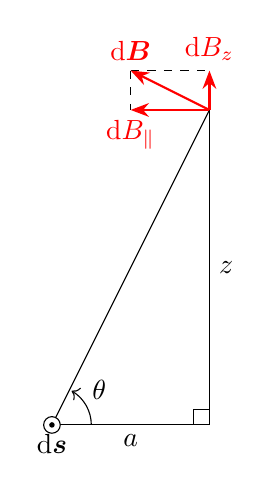
\begin{tikzpicture}
      \draw[thin](0,0)--(2,4);
      \draw[thin](0,0)--(2,0);
      \draw[thin](2,0)--(2,4);
      \draw[thin,dashed](1,4.5)--(2,4.5);      
      \draw[thin,dashed](1,4.5)--(1,4);
      \filldraw [fill=white] (0,0) circle [radius=3pt];
      \fill [fill=black] (0,0)circle [radius=1pt];
      \draw (0,0)node[below]{$\dd \bm{s}$};      
      \draw (1,0)node[below]{$a$};
      \draw (2,2)node[right]{$z$};
      \draw[thick,color=red,-Stealth](2,4)--(1,4.5)node[above]{$\dd \bm{B}$};
      \draw[thick,color=red,-Stealth](2,4)--(1,4)node[below]{$\dd B_{\parallel}$};
      \draw[thick,color=red,-Stealth](2,4)--(2,4.5)node[above]{$\dd B_{z}$};      
      \draw[thin](2,0.2)--(1.8,0.2)--(1.8,0);
      \draw [->](0.5,0) arc [start angle = 0, end angle = 60, radius = 0.5];
      \draw (0.6,0.2)node[above]{$\theta$};
    \end{tikzpicture}
    \caption{$\bm{r}-\bm{s}$と$\dd\bm{B}$の作る断面}    
    \label{cross_section}
  \end{figure}
  すると,$\bm{s}$に平行な成分は積分によって消えるので,$\bm{s}$に垂直な成分のみを考えればよい.よって,垂直成分$\dd B_{z}$は
  \begin{equation}
    \dd B_{z}
    =
    |\dd B|\cos \theta
    =
    \frac{\mu_{0}I}{4\pi}
    \cdot
    \frac{a |\dd \bm{s}|}{(a^2+z^2)^{3/2}}
  \end{equation}
  である.よって,
  \begin{equation}
    B_{z}
    =
    \int_{0}^{2\pi a}
    \frac{\mu_{0}I}{4\pi}
    \cdot
    \frac{a \dd s}{(a^2+z^2)^{3/2}}
    =
    \frac{\mu_{0}I}{2}
    \cdot
    \frac{a^2}{(a^2+z^2)^{3/2}}
  \end{equation}
  である.

  \item 
  $\hat{r}=\hat{n}$の場合を考えると,
  \begin{equation}
    \bm{B}
    =
    2K(r)IS\hat{r}
    =
    2\pi a^2K(r)I\hat{r}
  \end{equation}
  であり,これが前問の結果と一致するとすれば
  \begin{equation}
    2\pi a^2K(r)I\hat{r}
    =    
    \frac{\mu_{0}I}{2}
    \cdot
    \frac{a^2}{(a^2+r^2)^{3/2}}
  \end{equation}
  である.よって,これを$K(r)$について解けば
  \begin{equation}
    K(r)
    =
    \frac{\mu_{0}}{4\pi}\cdot\frac{1}{(a^2+r^2)^{3/2}}
  \end{equation}
  である.

  \item 
  磁気双極子$2$の作った磁場によって,磁気双極子$1$がポテンシャルエネルギーを持つような場合を考えればよい.磁気双極子$2$が作る磁場は
  \begin{equation}
    \bm{B}_{2}
    =
    -K(d)
    \left[ 
    \bm{m}_{2}
    -
    3(\bm{m}_{2}\cdot\hat{r})\hat{r}
    \right]
  \end{equation}
  なので,
  \begin{equation}
    U_{1}
    =
    -\bm{B}_{2}\cdot\bm{m_{1}}
    =
    K(d)m^2
    \left(
    \cos(\theta_{1}-\theta_{2})
    -
    3\cos\theta_{1}\cos\theta_{2}
    \right)
  \end{equation}
  である.これは,$(\theta_{1},\theta_{2})=(0,0),(\pi,\pi)$のときに最小である.

  \begin{itemize}
    \item
    \uline{$\theta_{1}=0$のとき}

    ポテンシャルは
    \begin{equation}
      U_{1}
      =
      -2K(d)m^2 \cos\theta_{2}
    \end{equation}    
    である.よって,$U_1$は図\ref{theta0}のようになる.
    
    \item 
    \uline{$\theta_{1}=\pi/2$のとき}

    ポテンシャルは
    \begin{equation}
      U_{1}
      =
      K(d)m^2 \sin\theta_{2}
    \end{equation}    
    である.よって,$U_1$は図\ref{thetapi2}のようになる.

    \begin{figure}[ht]
      \centering
        \begin{tabular}{cc}      
          \begin{minipage}[t]{0.3\linewidth}
            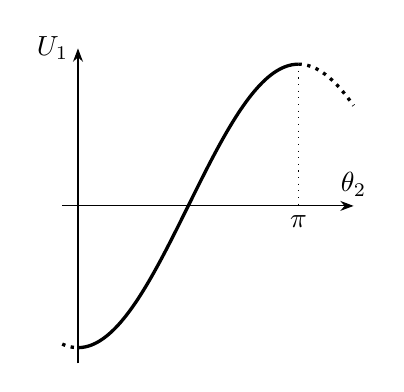
\begin{tikzpicture}
               \draw[thin,-Stealth] (-0.2,0)--(3.5,0)node[above]{$\theta_{2}$};
               \draw[thin,-Stealth] (0,-2)--(0,2)node[left]{$U_{1}$};
               \draw[very thick,samples=100,domain=-0:2.8]plot(\x,{-1.8*cos(\x*180/2.8)});
               \draw[very thick,samples=100,domain=-0.2:0,dotted]plot(\x,{-1.8*cos(\x*180/2.8)});
               \draw[very thick,samples=100,domain=2.8:3.5,dotted]plot(\x,{-1.8*cos(\x*180/2.8)});
               \draw [thin,dotted](2.8,1.8)--(2.8,0)node[below]{$\pi$};
            \end{tikzpicture}               
            \label{theta0}
            \caption{$\theta_{1}=0$のとき}
          \end{minipage} &
          \begin{minipage}[t]{0.3\linewidth}
            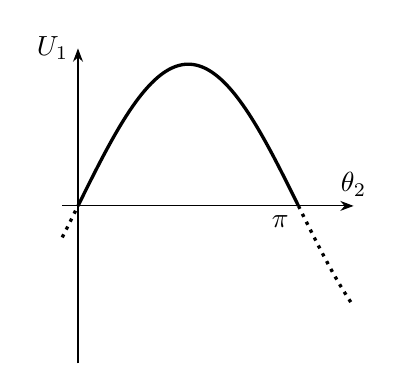
\begin{tikzpicture}
              \draw[thin,-Stealth] (-0.2,0)--(3.5,0)node[above]{$\theta_{2}$};
              \draw[thin,-Stealth] (0,-2)--(0,2)node[left]{$U_{1}$};
              \draw[very thick,samples=100,domain=-0:2.8]plot(\x,{1.8*sin(\x*180/2.8)});
              \draw[very thick,samples=100,domain=-0.2:0,dotted]plot(\x,{1.8*sin(\x*180/2.8)});
              \draw[very thick,samples=100,domain=2.8:3.5,dotted]plot(\x,{1.8*sin(\x*180/2.8)});
              \draw (2.8,0)node[below left]{$\pi$};
              \label{thetapi2}
            \end{tikzpicture}     
          \caption{$\theta_{1}=\pi/2$のとき}
        \end{minipage}
      \end{tabular}
    \end{figure}

  \end{itemize}

  \item 
  磁場の影響を加えれば
  \begin{align}
    U_{2}
    &=
    U_{1}-\bm{B}_{0}\cdot\bm{m}_{1}-\bm{B}_{0}\cdot\bm{m}_{2}
    \nonumber
    \\
    &=
    K(d)m^2
    \left(
    \cos(\theta_{1}-\theta_{2})
    -
    3\cos\theta_{1}\cos\theta_{2}
    \right)
    -B_{0}m_{1}\sin\theta_{1}
    -B_{0}m_{2}\sin\theta_{2}
    \nonumber
    \\
    &=
    -2K(d)m^2
    \cos\theta_{1}\cos\theta_{2}
    +
    K(d)m^2\sin\theta_{1}\sin\theta_{2}
    -
    B_{0}m\sin\theta_{1}
    -
    B_{0}m\sin\theta_{2}
  \end{align}
  となる.この$U_{2}$の変分を考えれば
  \begin{align}
    \delta U_{2}
    &=
    -2K(d)m^2
    \delta(\cos\theta_{1})\cos\theta_{2}
    -2K(d)m^2
    \cos\theta_{1}\delta(\cos\theta_{2})
    \nonumber
    \\
    &\hspace{1cm}
    +
    K(d)m^2\delta(\sin\theta_{1})\sin\theta_{2}
    +
    K(d)m^2\sin\theta_{1}\delta(\sin\theta_{2})
    \nonumber
    \\
    &\hspace{1cm}    
    -
    B_{0}m\delta(\sin\theta_{1})
    -
    B_{0}m\delta(\sin\theta_{2})    
    \nonumber
    \\
    &=
    \left\{ -\frac{1}{2}Km^2 + \frac{1}{2}B_{0}m \right\}\delta \theta_{1}^2
    +
    \left\{ -\frac{1}{2}Km^2 + \frac{1}{2}B_{0}m  \right\}\delta \theta_{2}^2
  \end{align}
  である.ただし,
  \begin{align}
    \delta (\cos\theta_{i})
    &=
    -\sin\theta_{i}\delta\theta_{i}
    -\frac{1}{2}\cos\theta_{i}\delta\theta_{i}^2
    \nonumber
    \\
    &=
    -\delta\theta_{i}
    \\
    \delta (\sin\theta_{i})
    &=
    \cos\theta_{i}\delta\theta_{i}
    -
    \frac{1}{2}\sin\theta_{i}\delta\theta_{i}^2
    \nonumber
    \\
    &=
    -\frac{1}{2}\delta \theta_{i}^2
  \end{align}
  を用いた.よって,$\delta U_{2}=0$となるためには,$\delta\theta_{i}^2$の係数が$0$である必要があるので
  \begin{equation}
    B_{0}
    =
    Km
  \end{equation}
  である.

\end{enumerate}

\clearpage
\prb{I}{3}{A}{物理数学}
\begin{enumerate}
  \item 
  固有方程式は
  \begin{equation}
    \begin{vmatrix}
      \lambda-3 & -2 \\
      -1 & \lambda-4
    \end{vmatrix}
    =
    \left( \lambda-2 \right)\left( \lambda-5 \right)
    =
    0
  \end{equation}
  なので,固有値は$\lambda=2,5$である.対応する固有ベクトルは
  \begin{equation}
    v_{1}
    =
    \begin{pmatrix}
      2 \\
      -1
    \end{pmatrix}
    \ ,\ \ 
    v_{2}
    =
    \begin{pmatrix}
      1 \\
      1
    \end{pmatrix}
  \end{equation}
  なので,
  \begin{equation}
    P
    =
    \begin{pmatrix}
      2 & 1 \\
      -1 & 1
    \end{pmatrix}
  \end{equation}
  とすれば,
  \begin{equation}
    P^{-1}
    =
    \frac{1}{3}
    \begin{pmatrix}
      1 & -1 \\
      1 & 2
    \end{pmatrix}
  \end{equation}
  であり,$P^{-1}AP$を計算してみると
  \begin{equation}
    D
    \coloneqq
    P^{-1}AP
    =
    \frac{1}{3}
    \begin{pmatrix}
      1 & -1 \\
      1 & 2
    \end{pmatrix}
    \begin{pmatrix}
      3 & 2 \\
      1 & 4
    \end{pmatrix}
    \begin{pmatrix}
      2 & 1 \\
      -1 & 1
    \end{pmatrix}
    =
    \begin{pmatrix}
      2 & 0 \\
      0 & 5
    \end{pmatrix}
  \end{equation}
  と対角化できていることに注意する.すると
  \begin{align}
    A^{n}
    &=
    PDP^{-1}
    \cdots
    PDP^{-1}
    \nonumber
    \\
    &=    
    \frac{1}{3}
    \begin{pmatrix}
      2 & 1 \\
      -1 & 1
    \end{pmatrix}
    \begin{pmatrix}
      2^n & 0 \\
      0 & 5^n
    \end{pmatrix}
    \begin{pmatrix}
      1 & -1 \\
      1 & 2
    \end{pmatrix}
    =
    \frac{1}{3}
    \begin{pmatrix}
      2^{n+1}+5^{n} & -2^{n+1}+2\cdot5^{n} \\
      -2^{n}+5^{n} & 2^{n}+2\cdot5^{n}
    \end{pmatrix}
  \end{align}
  である.

  \item 
  次の関数
  \begin{equation}
    L
    \coloneqq
    xyz
    -
    \lambda
    \left( \frac{x^2}{4}+\frac{y^2}{9}+z^2-1 \right)
  \end{equation}
  を考える.$L$の$x,y,z,\lambda$による偏微分を考え,それらが$0$であるとすれば
  \begin{align}
    yz-\frac{\lambda}{2}x&=0
    \label{eq1}
    \\
    xz-\frac{2\lambda}{p}y&=0
    \label{eq2}
    \\
    xy-2\lambda z&=0
    \label{eq3}
    \\
    \frac{x^2}{4}+\frac{y^2}{9}+z^2&=1
    \label{eq4}
  \end{align}
  となり,これらの解が最大値の候補となる.まず,\eqref{eq1}を$\lambda$について解くと
  \begin{equation}
    \lambda
    =
    \frac{2yz}{x}
  \end{equation}
  である.これらを\eqref{eq2},\eqref{eq3}に代入してそれぞれを$y,z$について整理すると
  \begin{equation}
    \frac{y^2}{9}
    =
    \frac{x^2}{4}
    \ ,\ \ 
    z^2
    =
    \frac{x^2}{4}
    \label{eq5}
  \end{equation}
  である.これらを\eqref{eq4}について代入すると
  \begin{equation}
    x^2
    =
    \frac{4}{3}
  \end{equation}
  となる.これを\eqref{eq5}に代入すれば
  \begin{equation}
    (x,y,z)
    =
    (\pm2/\sqrt{3},\pm\sqrt{3},\pm1/\sqrt{3})
  \end{equation}
  である.ただし,複号は任意である.よって,$F=xyz$が最大となるためには,これらを掛け合わせた値が正であるように符号をとってくれば良いだけなので,最大値は
  \begin{equation}
    F_{\max}
    =
    \frac{2}{\sqrt{3}}
  \end{equation}
  であり,それを実現する$(x,y,z)$は
  \begin{equation}
    (2/\sqrt{3},\sqrt{3},1/\sqrt{3})
    \ ,\ \ 
    (-2/\sqrt{3},-\sqrt{3},1/\sqrt{3})
    \ ,\ \ 
    (2/\sqrt{3},-\sqrt{3},-1/\sqrt{3})
    \ ,\ \ 
    (-2/\sqrt{3},\sqrt{3},-1/\sqrt{3})
  \end{equation}
  の$\dot{4\vphantom{\text{つ}}}\dot{\text{つ}}$である.

\end{enumerate}

\clearpage
\prb{I}{3}{B}{量子力学}
\begin{enumerate}
  \item 
  $N=a^{\dagger}a$として計算すると
  \begin{equation}
    \left[ 
    a^{\dagger}a
    ,
    a
    \right]
    =
    \left[ a^{\dagger},a \right]a
    =
    -a
  \end{equation}
  である.

  \item 
  前問と同様に計算すれば
  \begin{equation}
    \left[ a^{\dagger}a
    ,a^{\dagger} \right]
    =
    a^{\dagger}
  \end{equation}
  となる.
  
  \item 
  $\ev{n|a^{\dagger}a|n}$を2通りで計算すればよい.$N=a^{\dagger}a$として考えれば$N$であり,$a\ket{n}=c\ket{n-1}$として考えれば$c^2$となるので,$c>0$より,$c=\sqrt{n}$である.

  \item 
  それぞれの項を計算すれば
  \begin{align}
    \ev{\alpha|N^2|\alpha}
    &=
    \ev{\alpha|a^{\dagger}aa^{\dagger}a|\alpha}
    \nonumber
    \\
    &=
    \ev{\alpha|a^{\dagger}a^{\dagger}aa|\alpha}
    +
    \ev{\alpha|a^{\dagger}a|\alpha}
    \nonumber
    \\
    &=
    |\alpha|^4+|\alpha|^2
    \\
    \ev{\alpha|N|\alpha}
    &=
    \ev{\alpha|a^{\dagger}a|\alpha}
    \nonumber
    \\
    &=
    |\alpha|^2
  \end{align}
  なので,$\ev{\alpha|N^2|\alpha}-\ev{\alpha|N|\alpha}^2=|\alpha|^2$となる.
\end{enumerate}

\clearpage
\section{パート2}
\prb{II}{1}{\empty}{統計力学}
\begin{enumerate}
  \item 
  定義より
  \begin{equation}
    Z_{n-1}(s)
    =
    \sum_{s_{1}=\pm1}\cdots\sum_{s_{n-1}=\pm1}
    e^{\beta ss_{1}}\cdots e^{\beta s_{n-2}s_{n-1}}
    Z_{0}(s_{n-1})
  \end{equation}
  だが,$s_{1},\cdots,s_{n-1}$はただの和をとるための添え字なので\footnote{「最近の学生さんは,ダミー添え字とかいうんですかね.」},$s_{1},\cdots,s_{n-1}\rightarrow s_{2},\cdots,s_{n}$と添え字を書き直せば
  \begin{equation}
    Z_{n-1}(s_{1})
    =
    \sum_{s_{2}=\pm1}\cdots\sum_{s_{n}=\pm1}
    e^{\beta s_{1}s_{2}}\cdots e^{\beta s_{n-1}s_{n}}
    Z_{0}(s_{n})
  \end{equation}
  である.あとは,$Z_{n}(s)$の定義と比較して
  \begin{equation}
    Z_{n}(s)
    =
    \sum_{s_{n}=\pm1}e^{\beta ss_{1}}Z_{n-1}(s_{1})
  \end{equation}
  が示された.

  \item 
  $s=1$のときと,$s=-1$のときをそれぞれ書き下せば
  \begin{equation}
    \begin{dcases}
      zZ_{0}(1)
      &=
      e^{\beta}Z_{0}(1)+e^{-\beta}Z_{0}(-1)
      \\
      zZ_{0}(-1)
      &=
      e^{-\beta}Z_{0}(1)+e^{\beta}Z_{0}(-1)
    \end{dcases}
  \end{equation}
  なので,ここから$z$を消去すれば$Z_{0}(1)/Z_{0}(-1)=\pm1$となる.ここで,分配関数は正なので,複号は$+$をとれば,
  \begin{equation}
    z=2\cosh \beta
    \ ,\ \ 
    Z_{0}(1)/Z_{0}(-1)=1
  \end{equation}
  となる.

  \item 
  前問より,
  \begin{equation}
    Z_{n}
    =
    2^{n}\cosh^{n}\beta
  \end{equation}
  なので
  \begin{equation}
    S
    =
    -\pdv{F}{T}
    =
    \frac{nk_{B}}{J}\pdv{}{T}\left[ T\log2\cosh\left( \frac{J}{k_{B}T} \right) \right]
  \end{equation}
  であり,これを計算すれば
  \begin{equation}
    S
    =
    \frac{nk_{B}}{J}
    \left[ 
      \log2\cosh\left( \frac{J}{k_{B}T} \right)
      -
      \frac{J}{k_{B}T}\tanh\left( \frac{J}{k_{B}T} \right)
    \right]
  \end{equation}
  である.よって,イジングスピン1つあたりのエントロピー$s$は
  \begin{equation}
    s=\frac{S}{n}
    =
    \frac{k_{B}}{J}
    \left[ 
      \log2\cosh\left( \frac{J}{k_{B}T} \right)
      -
      \frac{J}{k_{B}T}\tanh\left( \frac{J}{k_{B}T} \right)
    \right]
  \end{equation}
  である.

  \item 
  (1)と同様に考えれば,$e^{\beta ss_{1}}Z_{n-1}^{\text{tree}}(s_{1})\times e^{\beta ss_{2}}Z_{n-1}^{\text{tree}}(s_{2})$の$Z_{n}^{\text{tree}}(s)$に対する寄与を考えればよい.よって
  \begin{equation}
    Z_{n}^{\text{tree}}(s)
    =
    \sum_{s_{1}=\pm1}\sum_{s_{2}=\pm2}e^{\beta ss_{1}}Z_{n-1}^{\text{tree}}(s_{1})\times e^{\beta ss_{2}}Z_{n-1}^{\text{tree}}(s_{2})
  \end{equation}
  である.

  \item 
  $s=1,-1$の場合をそれぞれ考えると
  \begin{equation}
    \begin{dcases}
      Z_{n}^{\text{tree}}(1)
      &=
      e^{2\beta}Z_{n-1}^{\text{tree}}(1)^2
      +
      2Z_{n-1}^{\text{tree}}(1)Z_{n-1}^{\text{tree}}(-1)
      +
      e^{-2\beta}Z_{n-1}^{\text{tree}}(-1)^2
      \\      
      Z_{n}^{\text{tree}}(-1)
      &=
      e^{-2\beta}Z_{n-1}^{\text{tree}}(1)^2
      +
      2Z_{n-1}^{\text{tree}}(1)Z_{n-1}^{\text{tree}}(-1)
      +
      e^{2\beta}Z_{n-1}^{\text{tree}}(-1)^2
    \end{dcases}
  \end{equation}
  なので
  \begin{equation}
    y
    =
    \frac{e^{2\beta}Z_{n-1}^{\text{tree}}(1)^2
    +
    2Z_{n-1}^{\text{tree}}(1)Z_{n-1}^{\text{tree}}(-1)
    +
    e^{-2\beta}Z_{n-1}^{\text{tree}}(-1)^2}{e^{-2\beta}Z_{n-1}^{\text{tree}}(1)^2
    +
    2Z_{n-1}^{\text{tree}}(1)Z_{n-1}^{\text{tree}}(-1)
    +
    e^{2\beta}Z_{n-1}^{\text{tree}}(-1)^2}
    =
    \left( \frac{ay+1}{y+a} \right)^2
  \end{equation}
  である.

  \item 
  $y$について解けば,
  \begin{equation}
    (y-1)(y^2-(a^2-2a-1)y+1)
    =
    0
  \end{equation}
  なので,$y$が$a$の関数だとすれば,$y^2-(a^2-2a-1)y+1=0$である.これを解くと
  \begin{equation}
    y=\frac{1}{2}\left\{ 
    a^2-2a-1
    \pm
    |a-1|\sqrt{(a-3)(a+1)}
    \right\}
  \end{equation}
  となる.このような解が存在するための条件は,$a=e^{2\beta}>0$と併せて考えると$a>3$なので
  \begin{equation}
    a_{c}
    =
    3
  \end{equation}
  である.

  \item 
  $a<a_{c}$では,系の状態は$y=1$しか存在しないが,$a>a_{c}$では可能な系の状態が$\dot{3\vphantom{\text{つ}}}\dot{\text{つ}}$となる.この$a_{c}$を\textbf{転移温度}とよぶ.
\end{enumerate}

\clearpage
\prb{II}{2}{\empty}{量子力学}
\begin{enumerate}
  \item 
  $\ket{L},\ket{R}$が基底を成しているので
  \begin{equation}
    \hat{H}
    =
    \begin{pmatrix}
      E_{0} & -K\\
      -K & E_{0}
    \end{pmatrix}
  \end{equation}
  である.

  \item 
  固有方程式は
  \begin{equation}
    \begin{vmatrix}
      \lambda-E_{0} & K \\
      K & \lambda-E_{0}
    \end{vmatrix}
    =
    (\lambda-E_{0})^2
    -
    K^2
    =
    0
  \end{equation}
  である.これを解けば$\lambda=E_{0}\pm K$である.基底状態に対応するのは$\lambda=E_{0}-K$であり,その状態は
  \begin{equation}
    \ket{0}
    =
    \frac{1}{\sqrt{2}}
    \begin{pmatrix}
      1 \\
      1
    \end{pmatrix}
  \end{equation}
  である.

  \item 
  前問より,第1励起状態は$\lambda=E_{0}+K$に対応し,その固有状態は
  \begin{equation}
    \ket{1}
    =
    \frac{1}{\sqrt{2}}
    \begin{pmatrix}
      1 \\
      -1
    \end{pmatrix}
  \end{equation}
  である.

  \item 
  これらの固有状態を用いれば,$\ket{L}=(1,0),\ket{R}=(0,1)$は
  \begin{equation}
    \begin{dcases}
      \ket{L}
      &=
      \frac{1}{\sqrt{2}}(\ket{0}+\ket{1})
      \\
      \ket{R}
      &=
      \frac{1}{\sqrt{2}}(\ket{0}-\ket{1})
    \end{dcases}
    \label{LR}
  \end{equation}
  である.これを逆に書けば
  \begin{equation}
    \begin{dcases}
      \ket{0}
      &=
      \frac{1}{\sqrt{2}}(\ket{L}+\ket{R})
      \\
      \ket{1}
      &=
      \frac{1}{\sqrt{2}}(\ket{L}-\ket{R})
    \end{dcases}
    \label{01}
  \end{equation}
  であることに注意しておく.時刻$t$での状態$\ket{\psi(t)}$について
  \begin{equation}
    \ket{\psi(t)}
    =
    \hat{a}(t)\ket{L}
    +
    \hat{b}(t)\ket{R}
  \end{equation}
  と書けば,シュレーディンガー方程式
  \begin{equation}
    i\hbar\pdv{}{t}\ket{\psi(t)}
    =
    \hat{H}\ket{\psi(t)}
  \end{equation}
  より,
  \begin{equation}
    \hat{a}(t)
    =
    Ae^{-i\hat{H}t/\hbar}
    \ ,\ \ 
    \hat{b}(t)
    =
    Be^{-i\hat{H}t/\hbar}
  \end{equation}
  であることがわかる.$t=0$では$\hat{a}(t)=1,\hat{b}(t)=0$なので
  \begin{equation}
    \hat{a}(t)
    =
    e^{-i\hat{H}t/\hbar}
    \ ,\ \ 
    \hat{b}(t)
    =
    0
  \end{equation}
  である.よって,
  \begin{equation}
    \ket{\psi(t)}
    =
    e^{-i\hat{H}t/\hbar}\ket{L}
    \label{state}
  \end{equation}
  と時間発展をあらわすことができた\footnote{物理的意味を考えれば\eqref{state}はすぐ出てくるので,試験ではそれでもいいかもしれない.}.よって,$\ket{L}$に\eqref{LR},\eqref{01}を用いれば
  \begin{align}
    \ket{\psi(t)}
    &=
    \frac{1}{\sqrt{2}}e^{-i\hat{H}t/\hbar}\ket{0}
    +
    \frac{1}{\sqrt{2}}e^{-i\hat{H}t/\hbar}\ket{1}
    \nonumber
    \\
    &=
    \frac{1}{\sqrt{2}}e^{-i(E_{0}-K)t/\hbar}\ket{0}
    +
    \frac{1}{\sqrt{2}}e^{-i(E_{0}+K)t/\hbar}\ket{1}
    \nonumber
    \\
    &=
    \frac{1}{2}e^{-i(E_{0}-K)t/\hbar}(\ket{L}+\ket{R})
    +
    \frac{1}{2}e^{-i(E_{0}+K)t/\hbar}(\ket{L}-\ket{R})
    \nonumber
    \\
    &=
    e^{-iE_{0}t/\hbar}\cos(Kt/\hbar)\ket{L}
    +
    ie^{-iE_{0}t/\hbar}\sin(Kt/\hbar)\ket{R}
  \end{align}
  となる.

  \item 
  規格化も考慮すれば
  \begin{equation}
    \ket{C}
    =
    \frac{1}{\sqrt{2}}
    (
      \ket{L}_{1}\otimes\ket{R}_{2}
      +
      \ket{R}_{1}\otimes\ket{L}_{2}
    )
  \end{equation}
  も基底になっている.

  \item 
  それぞれの行列要素を計算すれば
  \begin{equation}
    \begin{dcases}
      \ev*{A|\hat{H}|A}
      &=
      2E_{0}+U
      \\
      \ev*{A|\hat{H}|B}
      &=
      -2K
      \\
      \ev*{A|\hat{H}|C}
      &=
      -\sqrt{2}K
      \\
      \ev*{B|\hat{H}|B}
      &=      
      2E_{0}+U
      \\
      \ev*{B|\hat{H}|C}
      &=      
      -\sqrt{2}K
      \\
      \ev*{C|\hat{H}|C}
      &= 
      2E_{0}
    \end{dcases}
  \end{equation}
  なので,2粒子系のハミルトニアンは
  \begin{equation}
    \hat{H}
    =
    \begin{pmatrix}
      2E_{0} + U & -2K & -\sqrt{2}K \\
      -2K & 2E_{0} + U & -\sqrt{2}K \\
      -\sqrt{2}K  & -\sqrt{2}K & 2E_{0}
    \end{pmatrix}
  \end{equation}
  である.

  \item 
  固有値を計算すると,
  \begin{equation}
    2E_{0}+2K+U
    \ ,\ \ 
    2E_{0}-K+U\pm\sqrt{20K^2-4KU+U^2}
  \end{equation}
  である.よって,基底状態の固有エネルギーは,このなかでもっとも値の小さい
  \begin{equation}
    2E_{0}-K+U-\sqrt{20K^2-4KU+U^2}
  \end{equation}
  である.

\end{enumerate}

\end{document}
